\documentclass{article}

\usepackage[a3paper, margin=1cm]{geometry}
\newcommand{\dbtable}{\subsection}
\newcommand{\cmark}{\ding{51}}%
\newcommand{\mono}{\texttt}

\usepackage{booktabs}
\usepackage{pifont}
\usepackage{graphicx}
%\usepackage{tikz}


\begin{document}
	\section{Database}
	
	\textit{Note}: The original movies and series dataset contains the id's with the format \mono{tt\#\#\#\#\#\#\#}, since all the id's contains the "tt" string at the start, in this dummy system, for sake of simplicity we will omit that and assume the id is only the numerical characters in the string, hence the id's for some tables is no AutoIncremental. Also, no indexes or partitions will be created for the same reason.
	
	\textbf{Conventions}
	\begin{itemize}
		\item \textbf{Naming Conventions}:
			\begin{itemize}
				\item \textit{Tables}: All tables are named as follows \mono{TableName\_Role} where TableName is PascalCase and Role can take one of the following values Catalog, Master or Detail depending on the kind of data and relationships the table has.
				\item \textit{Columns}: All columns are named as follows \mono{column\_name[\_id]} where column\_name is snake\_case and \_id is included just in case the column is either a Primary Key or a Foreign Key.
				
			\end{itemize}
		
		\item \textbf{Acronyms and abbreviations}. Let it be understood by:
			\begin{itemize}
				\item \textit{PK}: Primary Key
				\item \textit{NN}: Not Null
				\item \textit{I}: Index
				\item \textit{UQ}: Unique
				\item \textit{AI}: Auto incremental
				\item \textit{UN}: Unsigned
				\item \textit{D}: Default				
			\end{itemize}
		
		\item \textbf{FK column} The FK column contains the following information, in that order and style:
		
			 \textbf{Table name}\mono{.Referenced column in the table}\newline
	\end{itemize}
	
	\textbf{System CRUD operations}
	\begin{itemize}
		\item \mono{INSERT}: NOT ALLOWED (only AND only when inserting all the data)
		\item \mono{DELETE}: NOT ALLOWED
		\item \mono{SELECT}: ALLOWED, on any table at any time
		\item \mono{UPDATE}: ALLOWED, just when updating movie or episode rating (and the corresponding cascade updates such as updating serie or season rating)
	\end{itemize}
	
	\dbtable{Movie\_Detail}
	\begin{table}[h!]
		\centering
		\begin{tabular}{|c|c|c|c|c|c|c|c|c|c|c|c|}
			\toprule
			\bfseries Column & \bfseries Data type & \bfseries Value range & \bfseries FK & \bfseries D & \bfseries PK & \bfseries NN & \bfseries I & \bfseries UQ & \bfseries AI & \bfseries UN & \bfseries Description\\
			
			\midrule
			id & \mono{INT} & default & & & \cmark & \cmark & \cmark & \cmark & & \cmark & The ID of the movie\\

			\midrule
			rating & \mono{DECIMAL(3,1)} & 0.0 - 10.0 & & 5.0 & & \cmark & & & & & The rating of the movie\\

			\midrule
			duration & \mono{SMALLINT} & default & & NULL & & &  & & & \cmark & The duration (in seconds) of the movie\\

			\midrule
			year & \mono{SMALLINT} & default & & & & \cmark & & & & \cmark & The year of the movie\\

			\midrule
			name & \mono{VARCHAR(100)} & & & & & \cmark & & & & & The name of the movie\\
			
			\midrule
			cover & \mono{VARCHAR(255)} & & & NULL & & & & & & & The file of the cover of the movie\\
			
			\midrule
			date\_inserted & \mono{TIMESTAMP} & & & & & \cmark & & & & & The \textit{CURRENT\_TIMESTAMP} when inserted (default)\\
			
			\bottomrule			
		\end{tabular}
	\end{table}
	\textit{rating} is Index 'cause we expect to query movies of certain rating, same goes for \textit{duration} and \textit{year}.
	
	The default value of rating is just arbitrary and can be changed.
	
	The default value of duration isn't arbitrary and SHOULD NOT be changed.
	

	\dbtable{Genre\_Catalog}
	\begin{table}[h!]
		\centering
		\begin{tabular}{|c|c|c|c|c|c|c|c|c|c|c|c|}
			\toprule
			\bfseries Column & \bfseries Data type & \bfseries Value range & \bfseries FK & \bfseries D & \bfseries PK & \bfseries NN & \bfseries I & \bfseries UQ & \bfseries AI & \bfseries UN & \bfseries Description\\
			
			\midrule
			id & \mono{TINYINT} & default & & & \cmark & \cmark & \cmark & \cmark & \cmark & \cmark & The ID of the genre\\
			
			\midrule
			genre & \mono{VARCHAR(50)} & & & & & \cmark & & \cmark & & & The name of the genre (e.g. horror)\\
			
			\bottomrule			
		\end{tabular}
	\end{table}

	\dbtable{Serie\_Detail}
	\begin{table}[h!]
		\centering
		\begin{tabular}{|c|c|c|c|c|c|c|c|c|c|c|c|}
			\toprule
			\bfseries Column & \bfseries Data type & \bfseries Value range & \bfseries FK & \bfseries D & \bfseries PK & \bfseries NN & \bfseries I & \bfseries UQ & \bfseries AI & \bfseries UN & \bfseries Description\\
			
			\midrule
			id & \mono{INT} & default & & & \cmark & \cmark & \cmark & \cmark & & \cmark & The ID of the serie\\
			
			\midrule
			year\_start & \mono{SMALLINT} & default & & & & \cmark & & & & \cmark & The year the tv serie started\\
			
			\midrule
			year\_end & \mono{SMALLINT} & default & & & & & & & & \cmark & The year the tv serie ended, NULL if it hasn't ended yet\\
			
			\midrule
			rating & \mono{DECIMAL(3,1)} & 0.0 - 10.0 & & 5.0 & & \cmark & & & & & The overall (average) rating of the seasons in this serie\\
			
			\midrule
			name & \mono{VARCHAR(100)} & & & & & \cmark & & & & & The name of the serie\\
			
			\midrule
			cover & \mono{VARCHAR(255)} & & & NULL & & & & & & & The file of the cover of the serie\\
			
			\midrule			
			date\_inserted & \mono{TIMESTAMP} & & & & & \cmark & & & & & The \textit{CURRENT\_TIMESTAMP} when inserted (default)\\
			
			\bottomrule
		\end{tabular}
	\end{table}

	\newpage
	\dbtable{Episode\_Detail}
	\begin{table}[h!]
		\centering
		\begin{tabular}{|c|c|c|c|c|c|c|c|c|c|c|c|}
			\toprule
			\bfseries Column & \bfseries Data type & \bfseries Value range & \bfseries FK & \bfseries D & \bfseries PK & \bfseries NN & \bfseries I & \bfseries UQ & \bfseries AI & \bfseries UN & \bfseries Description\\
			
			\midrule
			id & \mono{INT} & default & & & \cmark & \cmark & \cmark & \cmark & & \cmark & The ID of the episode\\
			
			\midrule
			serie\_id & \mono{INT} & default & \textbf{Serie\_Detail}\mono{.id} & & & \cmark & & & & \cmark & The id of the serie of that episode\\

			\midrule
			n\_episode & \mono{SMALLINT} & default & & & & \cmark & & & & \cmark & The number of the episode in the season\\
			
			\midrule
			n\_season & \mono{SMALLINT} & default & & & & \cmark & & & & \cmark & Number of the season, 0 is reserved for episodes with no season\\
			
			\midrule
			rating & \mono{DECIMAL(3,1)} & 0.0 - 10.0 & & 5.0 & & \cmark & & & & & The rating of the episode\\
			
			\midrule
			duration & \mono{SMALLINT} & default & & NULL & & & & & & \cmark & The duration (in seconds) of the episode\\
			
			\midrule
			name & \mono{VARCHAR(100)} & & & & & \cmark & & & & & The name of the episode\\
			
			\midrule
			cover & \mono{VARCHAR(255)} & & & NULL & & & & & & & The file of the cover of the episode\\
			
			\midrule			
			date\_inserted & \mono{TIMESTAMP} & & & & & \cmark & & & & & The \textit{CURRENT\_TIMESTAMP} when inserted (default)\\
			
			\bottomrule
		\end{tabular}
	\end{table}
	\textit{rating} is Index 'cause we expect to query episodes of certain rating, same goes for \textit{duration}.
	
	The default value of rating is just arbitrary and can be changed.
	
	The default value of duration isn't arbitrary and SHOULD NOT be changed.

	\dbtable{MovieGenres\_Master}
	\begin{table}[h!]
		\centering
		\begin{tabular}{|c|c|c|c|c|c|c|c|c|c|c|c|}
			\toprule
			\bfseries Column & \bfseries Data type & \bfseries Value range & \bfseries FK & \bfseries D & \bfseries PK & \bfseries NN & \bfseries I & \bfseries UQ & \bfseries AI & \bfseries UN & \bfseries Description\\
			
			\midrule
			movie\_id & \mono{INT} & default & \textbf{Movie\_Catalog}\mono{.id} & & & \cmark & \cmark & & & \cmark & The ID of the movie with certain genre\\
			
			\midrule
			genre\_id & \mono{TINYINT} & default & \textbf{Genre\_Catalog}\mono{.id} & & & \cmark & \cmark & & & \cmark & Id of the genre of the movie\\
			
			\bottomrule
		\end{tabular}
	\end{table}

	\dbtable{SerieGenres\_Master}
	\begin{table}[h!]
		\centering
		\begin{tabular}{|c|c|c|c|c|c|c|c|c|c|c|c|}
			\toprule
			\bfseries Column & \bfseries Data type & \bfseries Value range & \bfseries FK & \bfseries D & \bfseries PK & \bfseries NN & \bfseries I & \bfseries UQ & \bfseries AI & \bfseries UN & \bfseries Description\\
			
			\midrule
			serie\_id & \mono{INT} & default & \textbf{Serie\_Catalog}\mono{.id} & & & \cmark & \cmark & & & \cmark & The ID of the serie with certain genre\\
			
			\midrule
			genre\_id & \mono{TINYINT} & default & \textbf{Genre\_Catalog}\mono{.id} & & & \cmark & \cmark & & & \cmark & Id of the genre of the serie\\
			
			\bottomrule
		\end{tabular}
	\end{table}

	In the Figure~\ref{fig:relational-diagram} its shown the relational diagram for the database described above

	\begin{figure}
		\centering
		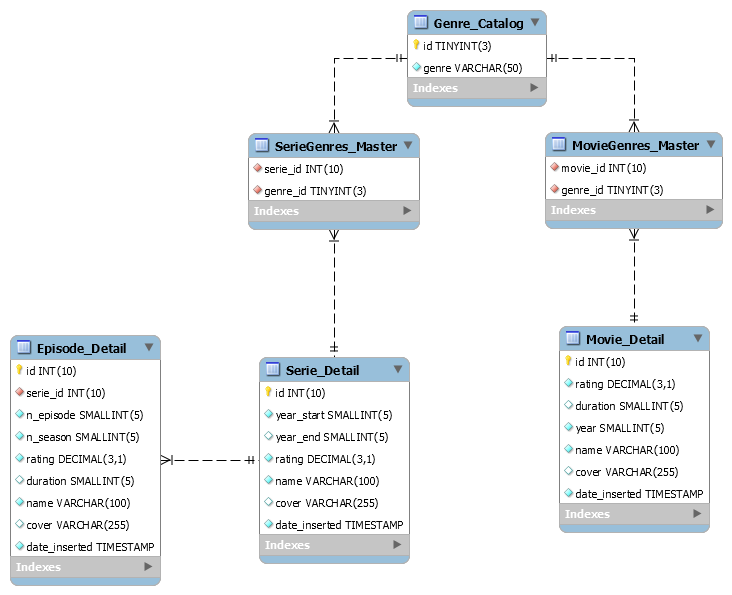
\includegraphics[width=0.75\linewidth]{OOPTecDummy-relational-diagram}
		\caption{Database relational diagram}
		\label{fig:relational-diagram}
	\end{figure}
\end{document}